\documentclass[12pt, twoside]{article}
\usepackage[letterpaper, margin=1in, head=30pt, headsep=0.1in]{geometry}
\usepackage[english]{babel}
\usepackage[utf8]{inputenc}
\usepackage{amsmath}
\usepackage{amsfonts}
\usepackage{amssymb}
\usepackage{tikz}
%\usetikzlibrary{quotes, angles}

\usepackage{graphicx}
\usepackage{enumitem}
\usepackage{multicol}

\newif\ifmeta
\metatrue %print standards and topics tags

\title{Regents Geometry}
\author{Chris Huson}
\date{October 2021}

\usepackage{fancyhdr}
\pagestyle{fancy}
\fancyhf{}
\renewcommand{\headrulewidth}{0pt} % disable the underline of the header
\raggedbottom


\fancyhead[LE]{\thepage}
\fancyhead[RO]{\thepage \\ Name: \hspace{4cm} \,\\}
\fancyhead[LO]{BECA / Dr. Huson / Geometry 03 Parallels and transversals}

\begin{document}

\subsubsection*{3.9 Exit Note Quiz: External angle theorem}
\begin{enumerate}
\item Do Not Solve. Circle the appropriate equation, cite a  justification:
  \begin{multicols}{2}
    \begin{itemize} 
      \item ``vertical $\angle$s are $\cong$" 
      \item ``definition of bisector" 
      \item ``linear pairs sum to $180^\circ$" 
      \item ``triangle external angle theorem''
      \item ``corresponding $\angle$s of $\parallel$ lines are $\cong$" 
      \item ``alternate interior $\angle$s are $\cong$"
      \item ``same-side interior $\angle$s are supplementary"
      %\item ``$\perp$ rays  with complementary $\angle$s adding to $90^\circ$" 
    \end{itemize}
  \end{multicols}
  \begin{enumerate}

    \item Given two parallel lines intersect a transversal, as shown. \hspace{1.5cm}
    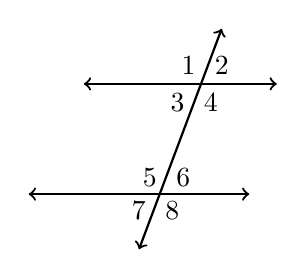
\begin{tikzpicture}[scale=0.7]
      \draw [<->, thick] (3,2)--(6.5,2);
      \draw [<->, thick] (2,0)--(6,0);
      \draw [<->, thick] (4,-1)--(5.5,3);
      \node at (4.5,0.3) [left]{$5$};
      \node at (4.5,0.3) [right]{$6$};
      \node at (4.3,-0.3) [left]{$7$};
      \node at (4.3,-0.3) [right]{$8$};
      \node at (5.2,2) [above left]{$1$};
      \node at (5.2,2) [above right]{$2$};
      \node at (5,2) [below left]{$3$};
      \node at (5,2) [below right]{$4$};
    \end{tikzpicture} \\[0.5cm]
    $\angle 2 \cong \angle 6$ \hspace{1cm} $m\angle 2 + m\angle 6 =  180$ \hspace{0.5cm} \rule{6cm}{0.15mm}
  
    \item Given $\overrightarrow{BA} \perp \overrightarrow{BC}$, with $\overrightarrow{BD}$ bisecting $\angle ABC$. \hspace{2cm}
      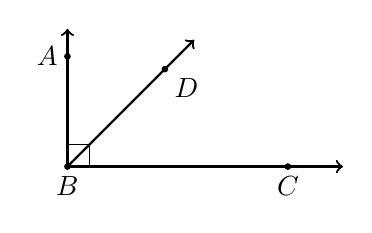
\begin{tikzpicture}[scale=0.7]
        \draw [<->, thick] (0,2.5)--(0,0)--(5,0);
        \draw [->, thick] (0,0)--(45:3.25);
        \draw [-, thin] (0, 0.4)--(0.4, 0.4)--(0.4, 0);
        \draw [fill] (0,0) circle [radius=0.05] node[below]{$B$};
        \draw [fill] (0,2) circle [radius=0.05] node[left]{$A$};
        \draw [fill] (4,0) circle [radius=0.05] node[below]{$C$};
        \draw [fill] (45:2.5) circle [radius=0.05] node[below right]{$D$};
      \end{tikzpicture}\\[0.5cm]
      $\angle ABD \cong \angle DBC$ \hspace{0.5cm} $m\angle ABD + m\angle DBC =  180$ \hspace{0.5cm} \rule{6cm}{0.15mm}
    
    \item $\overleftrightarrow{RPU}$ with ray $\overrightarrow{PS}$. \hspace{6cm}
    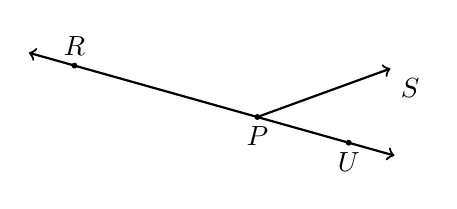
\begin{tikzpicture}[rotate=-10, scale=0.6]
      \draw [<->, thick] (-5,.5)--(3,-.3);
      \draw [->, thick] (0,0)--(30:3) node[below right]{$S$};
      \draw [fill] (0,0) circle [radius=0.05] node[below]{$P$};
      \draw [fill] (2,-0.2) circle [radius=0.05] node[below]{$U$};
      \draw [fill] (-4,0.4) circle [radius=0.05] node[above]{$R$};
    \end{tikzpicture}\\[0.5cm]
    $\angle RPS \cong \angle SPU$ \hspace{0.25cm} $m \angle RPS + m \angle SPU = 180^\circ$ \hspace{0.25cm} \rule{6cm}{0.15mm}  \vspace{0.25cm}

    \item Given $\triangle EFG$, with side extended as $\overrightarrow{EGH}$.\hspace{3cm}
    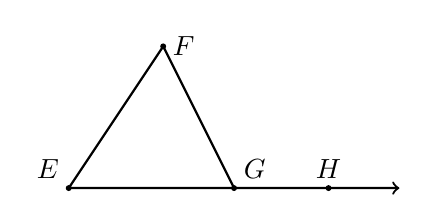
\begin{tikzpicture}[scale=0.6]
      %\draw [->, thick] (0,0)--(5,5);
      \draw [<-, thick] (8,0)--(1,0)--(3,3)--(4.5,0);
      \draw [fill] (1,0) circle [radius=0.05] node[above left]{$E$};
      \draw [fill] (4.5,0) circle [radius=0.05] node[above right]{$G$};
      \draw [fill] (3,3) circle [radius=0.05] node[right]{$F$};
      \draw [fill] (6.5,0) circle [radius=0.05] node[above]{$H$};
    \end{tikzpicture}\\[0.5cm]
    $\angle E \cong \angle F$ \hspace{0.5cm} $m\angle E + m\angle F =  m\angle FGH$ \hspace{0.5cm} \rule{6cm}{0.15mm} \vspace{0.25cm}

  \item Given $m \angle 1 = 4x+6$, $m \angle 2 = 6x-32$. Find $m \angle 1$.
  \hspace{2cm}
  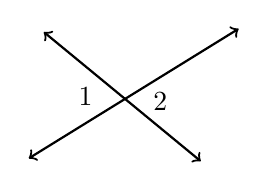
\begin{tikzpicture}[scale=.3, rotate=15]
    \draw [<->, thick] (0,-1.5)--(10,1.5);
    \draw [<->, thick] (2,3.5)--(7,-3.5);
    \node at (3,.4){1};
    \node at (6,-.6){2};
  \end{tikzpicture}\\[0.5cm]
  $\angle 1 \cong \angle 2$ \hspace{1cm} $m\angle 1 + m\angle 2 =  180$ \hspace{0.5cm} \rule{6cm}{0.15mm}
  \vspace{0.5cm}
\end{enumerate}

\newpage
\item Given $\triangle ABC$ with side $\overline{AC}$ extended through $D$ as shown. Find $x$ if $m\angle A=31$, $m\angle B=5x$, and $m\angle BCD=131$.
  \begin{flushright}
  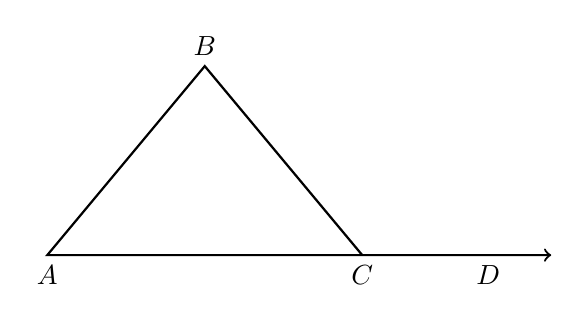
\begin{tikzpicture}[scale=0.8]
    %\draw [->, thick] (0,0)--(5,5);
    \draw [<-, thick] (8,0)--
      (7,0) node[below]{$D$}--
      (0,0) node[below]{$A$}--
      (2.5,3) node[above]{$B$}--
      (5,0) node[below]{$C$};
  \end{tikzpicture}
  \end{flushright} \vspace{2cm}
  
\item The measures in degrees of the three angles of a triangle are $2x$, $\frac{7}{6}x$, and $\frac{4}{3}x$. Find the measures of the triangle's angles. \vspace{5cm}

\item Given isosceles $\triangle JKL$ with $\overline{JL} \cong \overline{KL}$, and $m\angle J=5x-12$ and $m\angle K=3x+16$.
\begin{enumerate}
  \item Mark the congruent sides and angles of the triangle
  \item Find $m\angle L$
\end{enumerate}
\begin{flushright}
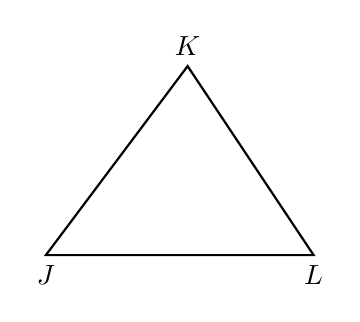
\begin{tikzpicture}[scale=0.8]
  %\draw [->, thick] (0,0)--(5,5);
  \draw [-, thick] (0,0) node[below]{$J$}--
    (2.25,3) node[above]{$K$}--
    (4.25,0) node[below]{$L$}--cycle;
\end{tikzpicture}
\end{flushright} \vspace{2cm}

\end{enumerate}
\end{document}